\documentclass[twoside=true, % doppelseitiger Druck
	DIV=15, % DIV Faktor für Satzspiegelberechnung, sie Doku zu KOMA Script
	BCOR=15mm, % Bindekorrektur
	chapterprefix=false,
	headinclude=true,
	footinclude=false,
	pagesize, % write pagesize to DVI or PDF
	fontsize=11pt, % use this font size
	paper=a4, % use ISO A4
	bibliography=totoc, % write bibliography-chapter to table of contents
	index=totoc, % write index-chapter to table of contents
	cleardoublepage=plain, % \cleardoublepage generates pages with pagestyle empty
	headings=big, % A4/B5
	listof=flat, % improved list of tables
	numbers=noenddot,
	parskip=half, % Absatz: durch Einrücken = false, Zeile = half / full (+, *, -)
]{scrbook}

% Zeilenabstand
\usepackage{setspace}
\setstretch{1.3}

\usepackage{scrhack}
\usepackage[utf8]{inputenc}
\usepackage{csquotes}
\usepackage{makeidx}
\usepackage{amsfonts}
\usepackage[slantedGreek,sc]{mathpazo} % Schriftart Palatino
% \usepackage{lmodern} % statt mathpazo, falls CM Fonts verwendet werden sollen
%\usepackage{mathptmx} % statt mathpazo, falls Times  verwendet werden soll
\usepackage[scaled=.95]{helvet}
\usepackage{courier}
\usepackage[T1]{fontenc}
\usepackage{textcomp}
\usepackage{amsmath} % standard math notation (vectors/sets/...)
\usepackage{bm} % standard math notation (fonts)
\usepackage{fixmath} % standard math notation (fonts)
\usepackage{graphicx}
\usepackage[facing=yes]{floatrow} % mehrere Gleitobjekte nebeneinander/caption neben Bild/Tabelle
\usepackage[labelfont=bf,sf,font=small,labelsep=space,format=plain]{caption}
\usepackage{subcaption}
\usepackage{scrpage2}
% \usepackage{pstool} % einbinden falls psfrag verwendet werden soll
\usepackage{epstopdf}
\usepackage[english]{babel}
\usepackage{ellipsis} % Korrigiert den Weißraum um Auslassungspunkte
\usepackage{microtype} % optischer Randausgleich etc.

%Zeilenumbruch für lange links swellnitz
\usepackage[hyphens]{url}

% Fußnoten werden jede Seite neu durchnummeriert
\usepackage{perpage} %the perpage package
\MakePerPage{footnote} %the perpage package command

% TIKZ: Um Schaubilder und Diagramme zu zeichnen
\usepackage{tikz}
\usetikzlibrary{arrows,automata}
% Blockbild-Test
\usetikzlibrary{shapes,arrows,shadows}
\usepackage{amsmath,bm,times}
\newcommand{\mx}[1]{\mathbf{\bm{#1}}} % Matrix command
\newcommand{\vc}[1]{\mathbf{\bm{#1}}} % Vector command

%Handling der Abkürzungen
\usepackage{acronym}

\usepackage{xcolor} % z.B. für schattierte Boxen
\usepackage{framed} % shaded Umgebung
\definecolor{shadecolor}{gray}{.85}%

% Links im PDF
\usepackage[colorlinks=false,
	pdfborder={0 0 0},
	breaklinks=true
]{hyperref}

% Lukas tabellen-spezifische pakete
\usepackage{graphicx}
\usepackage[normalem]{ulem}
\useunder{\uline}{\ul}{}
\usepackage{lscape}

% Kürzere Namen für \autoref
\addto\extrasngerman{
	\renewcommand{\sectionautorefname}{Abschnitt}
	\renewcommand{\subsectionautorefname}{Abschnitt}
	\renewcommand{\subsubsectionautorefname}{Abschnitt}
	\renewcommand{\figureautorefname}{Abb.}
	\renewcommand{\tableautorefname}{Tab.}
}


% Literaturangaben
\usepackage[
backend=biber,
style=alphabetic-verb, % numeric-verb oder alphabetic-verb
sorting=none,
backref=true
]{biblatex}
\addbibresource{thesis.bib}

% Features für Tabellen
\usepackage{multirow}
\usepackage{booktabs}
\usepackage{tabularx}
\usepackage{calc}
% Eigener Spaltentyp
\usepackage{array}
%% M: 1. Spalte: linksbündig, fett, 1.5cm breit
\newcolumntype{M}{>{\raggedright}p{4.5cm}}
%% M: 2. Spalte: linksbündig, fett, 1.5cm breit
\newcolumntype{N}{>{\raggedright}p{2.5cm}}
%% O: 3. Spalte: textbreite - 4 * spaltenrand - 1.5cm
\newcolumntype{O}{p{\textwidth-4\tabcolsep-7cm}}

%% R: 1. Spalte: rechsbündig, 1.5cm breit
\newcolumntype{R}{>{\raggedleft}p{1.5cm}}
%% S: 1. Spalte: rechsbündig, fett, 1.5cm breit
\newcolumntype{S}{>{\raggedleft\bfseries}p{1.5cm}}
%% T: 2. Spalte: textbreite - 4 * spaltenrand - 1.5cm
\newcolumntype{T}{p{\textwidth-4\tabcolsep-1.5cm}}

%% X: 1. Spalte: rechsbündig, 3.0cm breit
\newcolumntype{U}{>{\raggedleft}p{3.0cm}}
%% Y: 1. Spalte: rechsbündig, fett, 3.0cm breit
\newcolumntype{V}{>{\raggedleft\bfseries}p{3.0cm}}
%% Z: 2. Spalte: textbreite - 4 * spaltenrand - 3.0cm
\newcolumntype{W}{p{\textwidth-4\tabcolsep-3.0cm}}

%\typearea[current]{calc}

% Einstellungen für Bild-/Tabellenbeschriftung neben dem Bild
%\floatsetup[figure]{capbesideposition={inside,top}}
%\floatsetup[table]{capbesideposition={inside,top},style=plaintop}
\floatsetup[figure]{capbesideposition={inside,center}}
\floatsetup[table]{capbesideposition={inside,center},style=plaintop}
\renewfloatcommand{fcapside}{figure}[\capbeside][\FBwidth]
\newfloatcommand{tcapside}{table}[\capbeside][\FBwidth]

% für den \tab befehl
\usepackage{tabto}
\TabPositions{2cm,5cm,6.5cm,12cm}

\selectlanguage{english}

% Glossar, Akrynome, Abkürzungen
% http://tug.ctan.org/macros/latex2e/contrib/glossaries/glossariesbegin.pdf
% http://mirrors.rit.edu/CTAN/macros/latex/contrib/glossaries-extra/glossaries-extra-manual.pdf
% /usr/share/doc/texlive-doc/latex/glossaries-extra/glossaries-extra-manual.html
\usepackage[nonumberlist,toc=false]{glossaries-extra}
\setabbreviationstyle{long-short} % style
\makeglossaries % build glossaries for sorting with makeglossaries thesis
\loadglsentries{abbreviations} % load abbreviations from file

% Zur Darstellung von Quellcode
% https://en.wikibooks.org/wiki/LaTeX/Source_Code_Listings
\usepackage{listings}

% Standard style
\lstset{inputencoding=utf8,
    numbers=left,
	extendedchars=true,
	frame=single,
	showspaces=false,
	showstringspaces=false,
	showtabs=false,
	tabsize=4
}
% Eigener c style
\lstdefinestyle{customc}{
	belowcaptionskip=1\baselineskip,
	breaklines=true,
	frame=L,
	xleftmargin=\parindent,
	language=C,
	showstringspaces=false,
	basicstyle=\footnotesize\ttfamily,
	keywordstyle=\bfseries\color{green!40!black},
	commentstyle=\itshape\color{purple!40!black},
	identifierstyle=\color{blue},
	stringstyle=\color{orange},
}
% Eigener bash style
\lstdefinestyle{custombash}{
belowcaptionskip=1\baselineskip,
breaklines=true,
frame=L,
xleftmargin=\parindent,
language=bash,
showstringspaces=false,
basicstyle=\footnotesize\ttfamily,
keywordstyle=\bfseries\color{green!40!black},
commentstyle=\itshape\color{purple!40!black},
identifierstyle=\color{blue},
stringstyle=\color{orange},
}


\deffootnote{1em}{1em}{\makebox[1em][l]{\thefootnotemark}}

\makeindex

\newcommand{\real}{\mathord{\mathrm{I\!R}}}

\begin{document}
\selectlanguage{english}
\def\figdir{figures}
\def\tabledir{tables}
\def\picdir{pictures}
\def\srcdir{sourcecode}

\frontmatter
\pagestyle{scrplain}
\pagestyle{empty}
\begin{titlepage}

\sffamily

\raggedleft

\vspace*{-2cm}


\includegraphics{\figdir/logo-th-rosenheim-2018_master_quer_2c.eps}

\vfill

\centering
\LARGE
% \vspace*{\fill}
%-----------
Fakultät für Informatik  \vspace{0.5cm}\\
\Large
Studiengang Informatik

\vspace{2cm}

\LARGE

Attack surfaces and security measures in enterprise-level Platform-as-a-Service solutions

\vspace{2cm}

\Large
Bachelor Thesis

\vspace{1.5cm}


\Large
von

\vspace{0.5cm}

%\vspace*{\fill}

\LARGE
Lukas Grams

\vspace{1cm}

\vspace{1cm}

\flushleft
 \Large
\vspace*{\fill}

%-----------
\begin{tabbing}
Datum der Abgabe: \= tt.mm.2019 \kill
Datum der Abgabe: \> tt.mm.jjjj TODO \\
Erstprüfer: \> Prof.\ Dr.\ Reiner Hüttl\\
Zweitprüfer: \> Prof.\ Dr.\ Gerd Beneken
\end{tabbing}
%-----------

\end{titlepage}

\cleardoubleemptypage

{
\large
\thispagestyle{empty}
\vspace*{\fill}

\noindent
\textsc{Erklärung}

\medskip

\noindent
Ich versichere, dass ich diese Arbeit selbständig
angefertigt, nicht anderweitig für Prüfungszwecke
vorgelegt, keine anderen als die angegebenen Quellen
oder Hilfsmittel benützt sowie wörtliche und
sinngemäße Zitate als solche gekennzeichnet habe.

\bigskip

\noindent
Rosenheim, den tt.mm.jjjj TODO

\vspace*{2cm}

\noindent
Lukas Grams
}

%%% Local Variables: 
%%% mode: latex
%%% TeX-master: "d"
%%% End: 

% leere seite nach dem Deckblatt
\newpage\null\thispagestyle{empty}\newpage

%abstract
\chapter*{Kurzfassung (deutsch)}
\thispagestyle{empty}

TODO

\chapter*{Kurzfassung (englisch)}
\thispagestyle{empty}

TODO

\bigskip

\noindent
Schlagworte: 



\cleardoubleemptypage
\pagestyle{scrplain}
\pagenumbering{roman}
% ---------------------------------------------------
% D-TOC.TEX zur Verwendung mit TEXPART
% (an eigene Gegebenheiten anzupassen)
% ---------------------------------------------------
%
\setcounter{tocdepth}{1}
\tableofcontents
\clearpage
\listoffigures
\listoftables
\lstlistoflistings
% %style = super
\printglossary[style=super,title=List of abbreviations]
\cleardoublepage


\pagestyle{scrheadings}
\addtokomafont{caption}{\small}
\mainmatter
\chapter{Introduction}
With this chapter, the reader should be able to comprehend why this thesis was written, what it tries to accomplish and which topics are considered in this work.

\section{Motivation}

The increasing amount of Platform-as-a-Service (PaaS) solutions, cloud-hosted environments and
microservice architectures introduces new attack scenarios. This creates the need for new defense
strategies in both Development and Operations. Especially solutions providing (Kubernetes
conformant) container orchestration are identifiably different and in high demand compared to long
established solutions. This calls for a more detailed, focused examination. \\

\section{Objective}

This thesis aims to answer the following questions:

\begin{itemize}

\item What generic security risks emerge when providing or using a multi-tenant PaaS solution,
with each tenant developing, deploying and running their own applications? 

\item How can a PaaS provider (serving internal and/or external users) mitigate those risks? 

\item  In this scope and from a PaaS provider viewpoint, how does an on-premise solution compare
to a public cloud solution? 

\end{itemize}

Another goal is to recommend security measures for different implementation use cases.
If achievable within the provided time frame, it will additionally try and answer this question: 

\begin{itemize}

\item Does a cloud-hosted, self-managed solution (buy IaaS, provide PaaS) offer benefits in
contrast to the solutions compared above? \\
(In case there are sufficient differences, another set of security measures will be
recommended for this solution)

\end{itemize}


\section{Scope limitation}

To achieve the aforementioned goals, the view on the problem is limited to a manageable scope by
focusing on specific components of a few commonly used (Certified Kubernetes) PaaS solutions.
These components will be OpenShift Container Platform for On-Premise use cases and Azure Kubernetes Service as a public cloud solution. 
To include a cloud-hosted and self-managed solution, OpenShift running on self-managed instances in Azure serve as an
example implementation. \\
Components providing Kubernetes conformity will be the main focus, as these bear the most significance across all Kubernetes Certified solutions. \\
A look at popular tools and frameworks used in such clusters will be avoided in order to keep the scope manageable, though some might be recommended as a mitigation.\\
This thesis aims to provide insight to the risks of providing a PaaS solution and mitigations thereof. 
As such, it will look at the capabilities a potential provider has to (mis-)configure such solutions - inherent risks of the technologies themselves are only explored when measures to mitigate them are accessible from a provider standpoint. \\
In short, the goal is to improve the security of your Kubernetes cluster, not Kubernetes itself.\\
Looking at three common attack scenarios, it will then determine vulnerabilities and attack vectors,
as well as their potential damage and rate those risks:

\begin{itemize}

\item Malicious third party attacking the underlying infrastructure from within the LAN and/or the internet

\item Malicious third party attacking from inside a hijacked container, i.e. remotely executing code or commands

\item Bad user, i.e. a negligent, hijacked or malicious developer (account) risking compromise of his own and/or other applications

\end{itemize}

Possible measures to mitigate those risks will also be explored, evaluated and (if possible) put to use in the practical examples. 
With the results gathered, the thesis will compare different best practice implementations for different use cases and recommend measures for each.


TODO: Versioning Freeze! Openshift, AKS (not possible...), Docker engine, Kubernetes versions.

\chapter{Theory}
With this chapter, a reader with foundational knowledge of topics regarding Computer Science and/or Informatics should be able to grasp the specialized technologies discussed within the thesis and familiarize themselves with the definitions and terminology used throughout this thesis.

\section{Infrastructure-as-a-Service}
In \gls{iaas} environments, a consumer trusts his \gls{iaas} provider with the management and control of the infrastructure needed to deploy his applications.
The provided service ends at provisioning or processing, storage, networks and other computing resources \cite{nistcloud}
(TODO Quelle: https://nvlpubs.nist.gov/nistpubs/Legacy/SP/nistspecialpublication800-145.pdf ). 
Therefore consumers do not need to manage their own data centers or topics like system uplink availability.
As shown in Figure ~\ref{fig:servicecomparison}, consumers are responsible for the \gls{os} layer and everything above it.

(TODO: you manage <-> other manages https://www.bmc.com/blogs/saas-vs-paas-vs-iaas-whats-the-difference-and-how-to-choose/ )

citation test 1\cite{servicecomparison} \\
cit test 3~\cite{servicecomparison} \\
cit \citation{servicecomparison}

\begin{figure}[H]
\includegraphics[scale=0.4]{pictures/ServiceComparison.jpg} 
\caption{captionright\protect\footnotemark}
%% \caption{Comparison of responsibilities in different service models }
\label{fig:servicecomparison}
\end{figure}

\footnotetext{Source:  \cite{servicecomparison} }

\section{Platform-as-a-Service}

In \gls{paas} environments, a consumer trusts his \gls{paas} provider with the management and control of even more resources needed to deploy his applications beyond those covered by \gls{iaas}. 
(TODO Quelle: https://nvlpubs.nist.gov/nistpubs/Legacy/SP/nistspecialpublication800-145.pdf )
In an ideal scenario, this leads to a consumer not having to concern himself with the underlying network, hardware, servers, operating systems, storage or even common middleware like log data collection and analysis 
(TODO Quelle: https://docs.microsoft.com/en-us/azure/data-explorer/ )
 and allows him to focus on other tasks, i.e. application development. As a downside to this, a consumer might only have limited control on, among others, the software installed on the  machines provisioned. 
Although this shifts some of the responsibility burden towards the provider, the situation isn't as clear-cut as one might think. 
Figure X  (TODO: Picture link) shows middleware and runtime as provided, but there is no clear standard on what capabilities or tools are included.
A consumer might require capabilities which aren't provided or wishes to avoid provider lock-in through proprietary tools, again resulting in middleware responsibilities for the consumer. 
A consumer might also have to extensively configure the application-hosting environment for compliance or security purposes. 
Even some low-level tasks aren't completely managed, i.e. \gls{vm} reboots to apply security updates. 
(TODO Quelle: https://docs.microsoft.com/en-us/azure/aks/operator-best-practices-cluster-security?view=azuremgmtbilling-1.1.0-preview\#process-node-updates-and-reboots-using-kured )


\section{Containers, Docker}
TODO

concept of container vs. VM, upsides vs. downsides (?), docker-specific b/c highest market share
automation \& load elasticity -> need for orchestration

https://www.docker.com/resources/what-container\\
https://www.docker.com/sites/default/files/d8/2018-11/docker-containerized-and-vm-transparent-bg.png
Citations: TODO Look for books! 

\section{Container Orchestration}
TODO

idea: control system, architecture (control plane vs. application(s), kubelet, master/non-master nodes, ...), standard (can have other implementations), certification requirements, uses in general and in AKS/Openshift specifically.

\subsection{Kubernetes}

https://kubernetes.io/docs/concepts/\#overview \\
https://kubernetes.io/docs/concepts/overview/components/ \\
https://res.cloudinary.com/dukp6c7f7/image/upload/f\_auto,fl\_lossy,q\_auto/s3-ghost/2016/06/o7leok.png \\

\subsubsection{Kubernetes Objects}
TODO
higher-level idea behind objects
Pods, Services, Volumes, Namespaces

\subsubsection{Kubernetes Controllers}
TODO

higher-level idea behind controllers
ReplicaSets, Deployments, StatefulSets, DaemonSets, Jobs

\subsubsection{Using Kubernetes}
TODO

build from scratch, buy CaaS/PaaS/IaaS, cloud vs. on-prem, different scopes/features from different products

https://kubernetes.io/docs/setup/pick-right-solution/

\subsubsection{OpenShift}
TODO

\subsubsection{Azure Kubernetes Service}
TODO

\section{TODO: Others?}
TODO

\chapter{Risk Assessment of potential attack vectors}
TODO

\section{Defining procedures and approach}
Focus on three scenarios: attack through network, hijacked container, bad user

Research-Freeze: May 3rd, 2019! (Pre-KubeCon19, check git commit dates for stuff like OWASP-documents etc!)
Some newer information might be used for big outliers, but everything else just gets a side note

RISK ASSESSMENT METHODOLOGY:
difficulties with: 
A how generically should vectors be set?
B how to structure vectors (into categories?) 

Solution to A: vectors split and merged after risk assessment sketch; if there were considerable differences in the estimated values, they were split. If no diffs, they were merged.
Solution to B: Considerable time invested, no optimal solution was found. Ultimately ignored this, since more time investment wasnt feasible or added much value to the goals. TODO: Explain process, what was looked at and why it wasnt good, how we arrived at the end structure.

Risk assessment formula:
Risk = Probability * Impact.
Impact was taken as single value of 1 through 3  and estimated through None/Theoretical (0), Low/Intermediate-Step (1), non-severe security principle violation (2), severe security principle violation (3)

Probability was a bitch to define proberly. Therefore split into four factors: Vantage Point, Required Access Level (RAL), Detectability and Exploitability. Those initially had values between 0 though 3, but outlier values of 4  were defined for RAL and Vantage Point (in sync with existing assessment methodologies within HvS).
The average of these four values is taken as the total propability value, ranging from 0.25 through 3.5 (low <= 1.25, medium <= 2.25).
Vantage Point: physical access (0, see above since your own or the cloud providers hardware-accessing employees can also do whatever they want); node or management-interface (1); within container (2); within company network (3); from public www (4)
Required Access Level: cloud/infrastructure admin (0, since a rogue employee with super-admin can do whatever they want and this is about baseline security); cluster/system-admin (1); cluster/system user with read/write access (2); cluster/system user with read-only access (3); unauthenticated (4)
Detectability: Difficult (1) since it needs custom tools for environment-specific vuln detction; Average (2) since it is either generic but needs simple custom tools or its individualized but can be identified with some slight tool individualization; Easy (3) since there are generic script-kiddie tools / GUI-paths to find the vuln
Exploitability: Theoretical (0, since this is the level of unpublished 0-days and we are still doing baseline security); difficult (1) needs custom tools for environment-specific exploitation; Average(2), since its a generic exploit but needs simple custom tools or its inividualized but can be exploited with some slight tool individualization; Easy (3) since there are generic script-kiddie tools / GUI-paths to exploit the vuln

This leads to a total risk of 0 through 10.5, which is then rounded to one decimal place and capped at 10. In accordance to HvS internal models, total risk values <= 3 are defined as low, <= 6 as medium and values above that are defined as high.

specific values for each vector are estimated in a context with multiple assumptions:
- Tenants are only divided by namespace, NOT cluster!
- Default configs are used for everything, or just enough is changed to get the system functional, not secured!
- Average "usual" (non container-specific) application security measures have been taken (i.e. against the OWASP Top 10)
- The people administering and using the cluster (devs, cloud administrators, devops and their superiors) are familiar with conventional security principles and measures taken to secure solutions of moderate importance (read: not online banking, no industry-specific compliance requirements. i.e. simple networking and host security without many functionality restrictions)
- Those people are new to orchestrated container solutions and maybe containers + cloud solutions in general

- If multiple techniques can be used / impacts can occur to leverage a vector, all factor values of the one with the highest total risk are taken
- Values might decrease through the implementation of security measures, leading to a lower total value. (If multiple techniques could be used to leverage a vector and only one gets its total risk reduced, the new maximum risk value of that vector becomes the vector value(s)

goal is to reduce values above threshold X to below threshold X by applying security measures. This aims to ensure a basic security level, not something against APT groups / zero-day protection / targeted attacks with a lot of resources and competence. (no online banking, user data of average confidentiality etc)

Default values are defined as the following:

SETUP OF PRACTICAL PART:

Version freeze:
OpenShift Container Platform 3.11 -> OKD 3.11 ->  k8s-version = 1.11(.0 with fixes, is a fork. see: https://github.com/openshift/origin/releases/tag/v3.11.0 )
AKS (on May 3rd 2019) => k8s-version <= v1.13.5 available, but only for k8s-v1.11 only 1.11.8 or 1.11.9!

Considerable changes between 1.11.0 and 1.11.9 (Source: https://github.com/kubernetes/kubernetes/blob/master/CHANGELOG-1.11.md):
- action required: the API server and client-go libraries have been fixed to support additional non-alpha-numeric characters in UserInfo "extra" data keys. Both should be updated in order to properly support extra data containing "/" characters or other characters disallowed in HTTP headers. (#65799, @dekkagaijin)
- https://github.com/kubernetes/autoscaler/releases/tag/cluster-autoscaler-1.3.1
- ACTION REQUIRED: Removes defaulting of CSI file system type to ext4. All the production drivers listed under https://kubernetes-csi.github.io/docs/Drivers.html were inspected and should not be impacted after this change. If you are using a driver not in that list, please test the drivers on an updated test cluster first. ``` (#65499, @krunaljain)
- kube-apiserver: the Priority admission plugin is now enabled by default when using --enable-admission-plugins. If using --admission-control to fully specify the set of admission plugins, the Priority admission plugin should be added if using the PodPriority feature, which is enabled by default in 1.11. (#65739, @liggitt)
The system-node-critical and system-cluster-critical priority classes are now limited to the kube-system namespace by the PodPriority admission plugin. (#65593, @bsalamat)

no major changes => OCP 3.11, AKS-k8s 1.11.9!

Dependency compatibilities:
OCP 3.11: docker 1.13, CRI-O 1.11 (Source: https://docs.openshift.com/container-platform/3.11/release_notes/ocp_3_11_release_notes.html#ocp-311-about-this-release)
k8s-1.11: docker 1.11.2 to 1.13.1  (Source: https://github.com/kubernetes/kubernetes/blob/master/CHANGELOG-1.11.md#external-dependencies), CRI-O 1.11 (in-synch to k8s releases, source: https://github.com/cri-o/cri-o)
Azure-AKS: uses moby, NOT docker! (moby = pluggable container runtime based on docker, automatically updated in background whenever no node restart needed)

-> take defaults for all dependencies on install, document and apply all AKS node updates needing manual restart!
TODO: apply OCP updates when incoming?

\section{Identified vectors}

\subsection{Reconaissance through k8s control plane \& cloud provider interfaces}
Gather information useful for further attacks through interfaces intended to be accessible: the Kubernetes dashboard & apiserver as well as potential cloud provider webinterfaces & apiserver(s)
TODO

\subsection{Read confidentials through k8s control plane interfaces (dashboard, apiserver)}
Gather confidential information through the Kubernetes dashboard & apiserver (cloud provider interfaces are separately evaluated)
TODO

\subsection{Change configuration through k8s control plane interfaces}
Change the existing configuration through the Kubernetes dashboard & apiserver (cloud provider interfaces are separately evaluated)
TODO

\subsection{Read confidentials through cloud provider interfaces (mgmt console/API)}
Gather confidential information through potential cloud provider webinterfaces & apiserver(s) (Kubernetes interfaces are separately evaluated)
TODO

\subsection{Change configuration through  cloud provider interfaces (mgmt console/API)}
Change the existing configuration through potential cloud provider webinterfaces & apiserver(s) (Kubernetes interfaces are separately evaluated)
TODO

\subsection{Compromise internal k8s control plane components (etcd, scheduler, controller-manager)}
This vector comprises reconaissance, leaks of confidentials and configuration changes though Kubernetes components not intended to be accessible: etcd stores, kube-scheduler and kube-controller-manager
TODO

\subsection{Supply compromised container (base) image}
Supplying a malicious container image leading to security violations on the cluster (remote access for an attacker, resource misuse, data leakage, …). Most easily done untargeted (dockerhub images or dockerfiles on tutorials/help forums), but can be done targeted, too.
TODO

\subsection{Supply compromised k8s configuration}
Supplying a malicious kubernetes configuration leading to security violations on the cluster (remote access for an attacker, resource misuse, data leakage, …). Most easily done untargeted (tutorials/ help forums), but can be done targeted, too.
TODO

\subsection{compromise application components (lateral movement from container)}
Once an attacker gains access to a container, he may try to access more lucrative application components, i.e. databases or containers with more confidential information/traffic.
TODO

\subsection{R/W \& breakout to host, Privilege Escalation}
Once inside a container, an attacker may try to gain access to the underlying host by a multitude of means. This includes invoking syscalls, accessing the host file system and elevation priviledges within or outside of the container environment
TODO

\subsection{compromise local image cache}
If the cached image of a container can be manipulated, a functionally identical container, which violates security principles, could be started.
TODO

\subsection{modify running container}
Once inside a container, an attacker may try to modify the container to exfiltrate data or better suit their needs for further intrusion
TODO

\subsection{misuse node resources (DOS, cryptojacking)}
The resources of a single node are used to run a container and may be misconfigured or misused for financial gains (mining cryptocurrencies) or to disrupt service availability (i.e. through fork bombing or misconfiguration)
TODO

\subsection{hoard orchestration resources (DOS)}
The resources of the whole cluster may be misconfigured or misused to disrupt service availability (i.e. through fork bombing or misconfiguration)
TODO

\subsection{misuse orchestration resources (cryptojacking)}
The resources of the whole cluster may be misconfigured or misused for financial gains (mining cryptocurrencies)
TODO

\subsection{add malicious container}
A malicious container me be started within the cluster
TODO

\subsection{add malicious node}
A malicious node may be added to the cluster
TODO

\subsection{Bad user practice (outside of cluster)}
This vector comprises user practices outside of the cluster that lead to risks within it. Examples include phishing, openly publishing keys/tokens to public code repositories and more.
TODO

\subsection{Incufficient base infrastructure hardening}
The underlying nodes could allow an attacker easy entry, even if the containers themselves are hardened
TODO

\subsection{Entry through known, unpatched vulnerabilities}
Every system has to be kept up to date with  security patches. Publicly known vulnerabilities might otherwise be exploited, leading to potentially devastating violations of security principles
TODO

\section{PaaS solution risk analysis}
TODO

\subsection{Analysis results}
TODO: Risk analysis values here
TODO

\subsection{On-premise and public cloud environment comparison}
TODO: Comments on onPrem vs. cloud
TODO

\subsection{Multi-tenant isolation}
TODO: Comments on multi-tenant usage
TODO

\chapter{Best-Practice implementations}
TODO

\section{On-premise environment}
TODO

\subsection{Measure recommendations}
TODO: Includes comments on resulting (reduced) risk values!
TODO

\subsection{Practical examples}
TODO

\section{Public cloud environment}
TODO

\subsection{Measure recommendations}
TODO: Includes comments on resulting (reduced) risk values!
TODO

\subsection{Practical examples}
TODO

\chapter{Summary}
TODO: Include outlook with rootless builds, federated clusters (see: Google Anthos) and more!
TODO


%TEMPLATE TO CHOOSE FROM STARTS HERE%

\chapter{Einleitung}
\section{Anführungszeichen, Zitieren, Fußnoten} 
\label{kap:beschda}
Quellen stehen in der Datei thesis.bib!\\
Da gibt es auch ein tag, um Bücher von Online-Quellen zu unterscheiden.\\

So wird zitiert\cite{booktest}. Das ist eine Quelle für Bücher. \\
Das ist eine Online-Quelle\cite{wikimoscow}.
Um kleine Definitionen zu verlinken benutze ich Fußnoten\footnote{\url{ https://www.eclipse.org/4diac/} (Abgerufen am 07.02.2019)}

So werden in Deutschland Anführungszeichen gemacht: \glqq Sehr wichtig!!\grqq{}  \\

Die Abkürzungen stehen in der Datei abbreviations.tex! \\
Das abkürzungsverzeichnis wird natürlich automatisch erstellt.\\

So eine \gls{led} ist schon toll.

\begin{figure}[H]
\includegraphics[scale=0.5]{pictures/GatewayKommunikation.png} 
\caption{Bild wird automatisch im Abbildungsverzeichnis eingefügt!}
\label{fig:gateway}
\end{figure}


\chapter{Einführung und Analyse der Anforderungen}
Die Abbildung \ref{fig:archgrob} zeigt...
\begin{figure}[H]
\includegraphics[scale=0.3]{pictures/Architektur-grob.png} 
\caption{Bild wird automatisch im Abbildungsverzeichnis eingefügt!}
\label{fig:archgrob}
\end{figure}


\section{Tabelle und Liste}

Hier gibts eine Fancy Tabelle:\\
\begin{table}[H]
\begin{tabularx}{\textwidth}{| c | X | X | c |}	\hline	
\textbf{Nr.} & \textbf{Anforderung} & \textbf{Erklärung} & \textbf{Priorisierung} \\ 
\hline	
(1a) & Einfache Installation & einfache \glqq Out-of-the-box\grqq{} Installation und intuitives Anlegen von Nutzerkonten & Must \\
\hline 
\end{tabularx}
\renewcommand{\arraystretch}{1}\\	
\caption{Anforderungen an die Sprachsteuerung} 	
\label{tab:anfsprachsteuerung}
\end{table}


Liste um alles etwas in die Länge zu strecken:
\begin{itemize}\itemsep0pt
	\item Blah
	\item Blah
\end{itemize}

Bilder:

\begin{figure}[H]
\includegraphics[scale=0.3]{pictures/4diac.png} 
\caption{Bild wird automatisch im Abbildungsverzeichnis eingefügt!}
\label{fig:4diaclogo}
\end{figure}

\begin{figure}[H]
\includegraphics[scale=1]{pictures/IEC61499Modelle.png} 
\caption{Bild wird automatisch im Abbildungsverzeichnis eingefügt!}
\label{fig:iecwiki}
\end{figure}


\chapter{Automat mit tikz}

Falls jemand bock hat einen Automaten zu basteln, hier ist eine kleine Vorlage:

%siehe http://texample.net/tikz/examples/state-machine/

\begin{figure}[H]
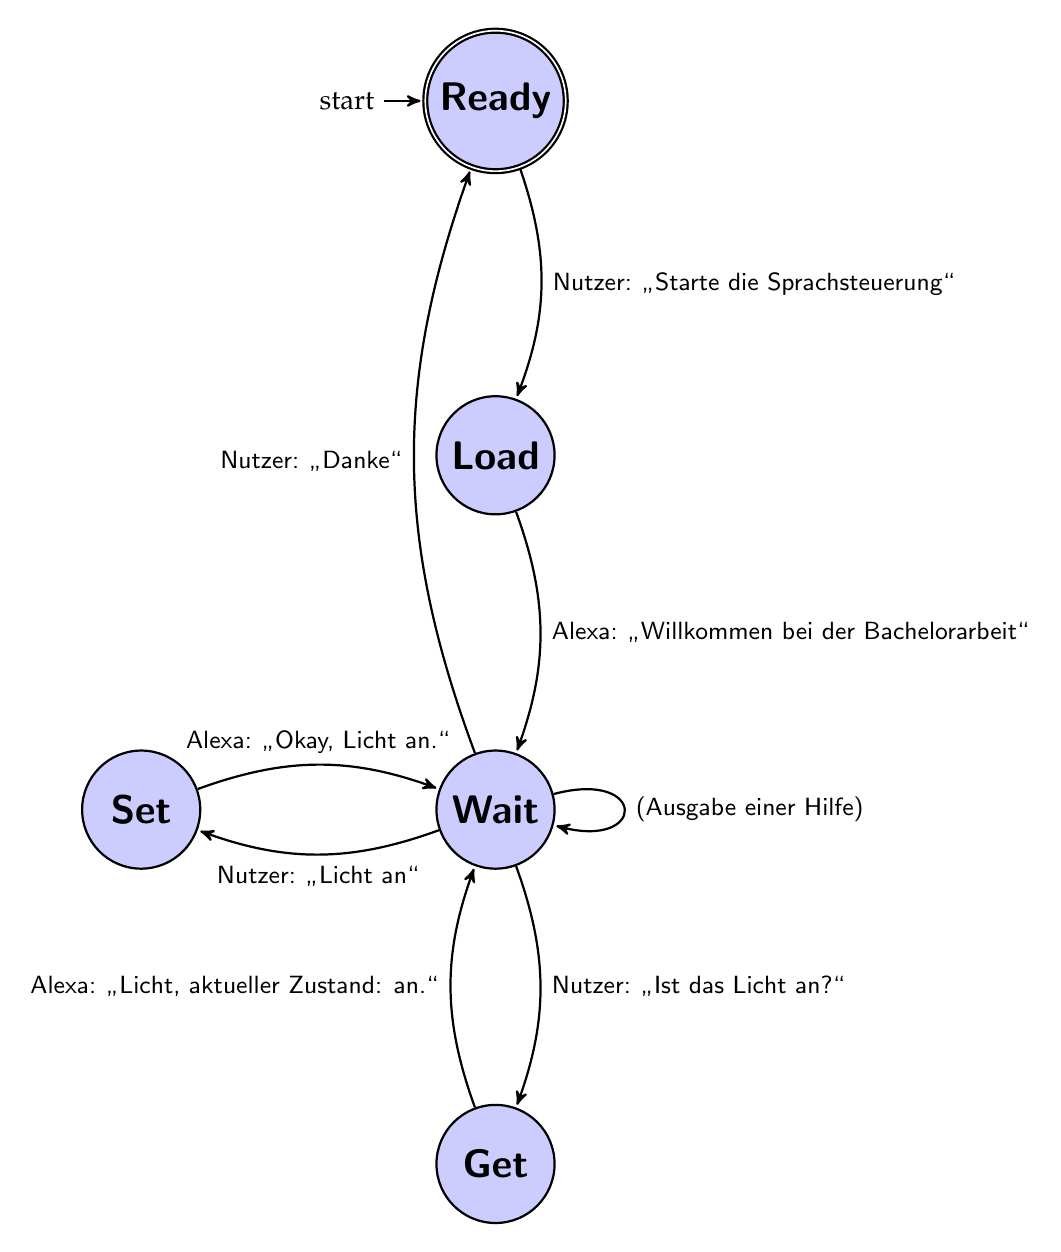
\begin{tikzpicture}[->,>=stealth',shorten >=1pt,auto,node distance=4.5cm,
 thick,state/.style={circle,fill=blue!20,draw,
 font=\sffamily\Large\bfseries,minimum size=15mm}]

 \node[state,initial,accepting] (AlexaReady) {Ready};
 \node[state] (Welcome) [below of=AlexaReady] {Load};
 \node[state] (Wait) [below of=Welcome] {Wait};
 \node[state] (set) [left of=Wait] {Set};
 \node[state] (get) [below of=Wait] {Get};


 \path[every node/.style={font=\sffamily\small,
 		fill=white,inner sep=1pt}]
 (AlexaReady) edge [bend left=20] node[right=1mm] {Nutzer: \glqq Starte die Sprachsteuerung\grqq{}} (Welcome)
 (Welcome) edge [bend left=20] node[right=1mm] {Alexa: \glqq Willkommen bei der Bachelorarbeit\grqq{}} (Wait)

 (set) edge [bend left=20] node[above=1mm] {Alexa: \glqq Okay, Licht an.\grqq{}} (Wait)
 (Wait) edge [bend left=20] node[below=1mm] {Nutzer: \glqq Licht an\grqq{}} (set)

 (get) edge [bend left=20] node[left=1mm] {Alexa: \glqq Licht, aktueller Zustand: an.\grqq{}} (Wait)
 (Wait) edge [bend left=20] node[right=1mm] {Nutzer: \glqq Ist das Licht an?\grqq{}} (get)

 (Wait) edge [bend left=20] node[left=1mm] {Nutzer: \glqq Danke\grqq{}} (AlexaReady)
 (Wait) edge [loop right] node[right=1mm] {(Ausgabe einer Hilfe)} (Wait);
 
\end{tikzpicture}
\caption{Automat des dialogbasierten Alexa Skill}
\label{fig:alexa-automat}
\end{figure}

\subsection{verlinken}

Verlinken mit Abbildungsnummer und Seite: \\
In der Abbildung \ref{fig:alexa-automat} auf Seite \pageref{fig:alexa-automat} wird gezeigt wie nice tikz sein kann.


\chapter{Listings}

Immer nice, Listings mit Synthax-Highlighting!\\

\lstinputlisting[style=custombash, firstline=31, lastline=48,
caption={Datei: setup-posix-mqtt.sh, Zeilen 31-48},
label={fig:setupmqtt}
]{sourcecode/setup-posix-mqtt.sh}

So wird verlinkt: \\

Das \autoref{fig:setupmqtt} auf Seite \pageref{fig:setupmqtt} zeigt in den Zeilen 34 bis 56 wie hässlich ein Shellscript werden kann. Hier wurde der Style custombash verwendet. Im \autoref{lst:skilllaunch} auf Seite \pageref{lst:skilllaunch} wird der customc-Style verwendet.


\lstinputlisting[style=customc,
caption={IntentHandler für den LaunchRequest},
label={lst:skilllaunch}
]{sourcecode/index-launchRequest.js}


% Literaturangaben
\printbibheading
\printbibliography[keyword={book},heading=subbibliography,title={Books}]
\printbibliography[keyword={online},heading=subbibliography,title={Online text-based sources}]
\printbibliography[keyword={video},heading=subbibliography,title={Online video sources}]
\printbibliography[keyword={Misc},heading=subbibliography,title={Other sources}]
\cleardoublepage

\end{document}
